\documentclass{scrbook}
\usepackage{graphicx} % Required for inserting images
\usepackage{tabularx} % Required for fixed width tables
\usepackage{scrlayer-scrpage} % Required for the subtitles
\usepackage{url} % Required for the URLs
\usepackage{hyperref} % Required for the URLs
\usepackage{listings} % Required for the code snippets
\usepackage{mathtools} % Required for the system of equations
\usepackage{amsmath,amssymb} % Required for some math symbols
\usepackage{enumitem} % Required for lettered lists

% Put the caption of the snippets at the bottom
\lstset{
    captionpos=b
}


\title{Blockchain data structures}
\subtitle{Ambient intelligence course (A.Y. 2025/2026)\\Topic taught by Prof. Arnaldo Tomasino}
\author{Gabriele Colapinto}
\date{\today}

\begin{document}

\maketitle
\thispagestyle{empty}

{\Large\textbf{License}} \\
{Notes from Ambient intelligence (A.Y. 2025/2026) by Gabriele Colapinto. 
Course taught by professors Michele Ruta, Floriano Scioscia, Arnaldo Tomasino, Davide Loconte — 
Licensed under CC BY-NC 4.0.\\
\url{https://creativecommons.org/licenses/by-nc/4.0/}}

\vspace*{\fill}
\rule{\textwidth}{0.2pt}
\small{© 2025 Gabriele Colapinto \\
Released under the \href{https://creativecommons.org/licenses/by-nc/4.0/}{Creative Commons Attribution–NonCommercial 4.0 International License}}

\clearpage

\tableofcontents

\chapter{Core Blockchain Data Structures and Network Architecture}

\section{The Anatomy of a Blockchain: Blocks and Transactions}

The integrity and functionality of a blockchain derive from its core data structures: the transactions that encapsulate state changes and the blocks that aggregate these transactions into a cryptographically secured, linear history. Each block acts as a container for a batch of transactions that have been validated by the network.\\

The structure of a single block consists of two primary components: a header and a list of transactions. (See figure ~\ref{fig:blockchain})\\

\begin{itemize}
    \item \textbf{Block Header:} A compact summary of the block's content, which includes several critical fields:
    \begin{itemize}
        \item \textit{Block Hash:} The unique cryptographic hash of the block header itself, serving as the block's identifier.
        \item \textit{Previous Block Hash:} A cryptographic hash of the preceding block's header. This is the crucial link that forms the "chain," ensuring the sequence and integrity of the entire ledger.
        \item \textit{Timestamp:} The time at which the block was created, providing a chronological order to the ledger.
        \item \textit{Nonce:} A value used in the proof-of-work calculation. Miners repeatedly change the nonce to find a block hash that meets the network's difficulty requirements.
        \item \textit{Merkle Root:} The root hash of the Merkle tree, which is a cryptographic summary of all the transactions included in the block.
    \end{itemize}
    \item \textbf{List of Transactions:} The payload of the block, containing the collection of all transactions that have been validated and included.
\end{itemize}

The design of these blocks provides the foundation for the ledger's security, but the method used to structure the transactions within them is equally important, leading to two primary models for managing value and ownership.

\begin{figure}
    \centering
    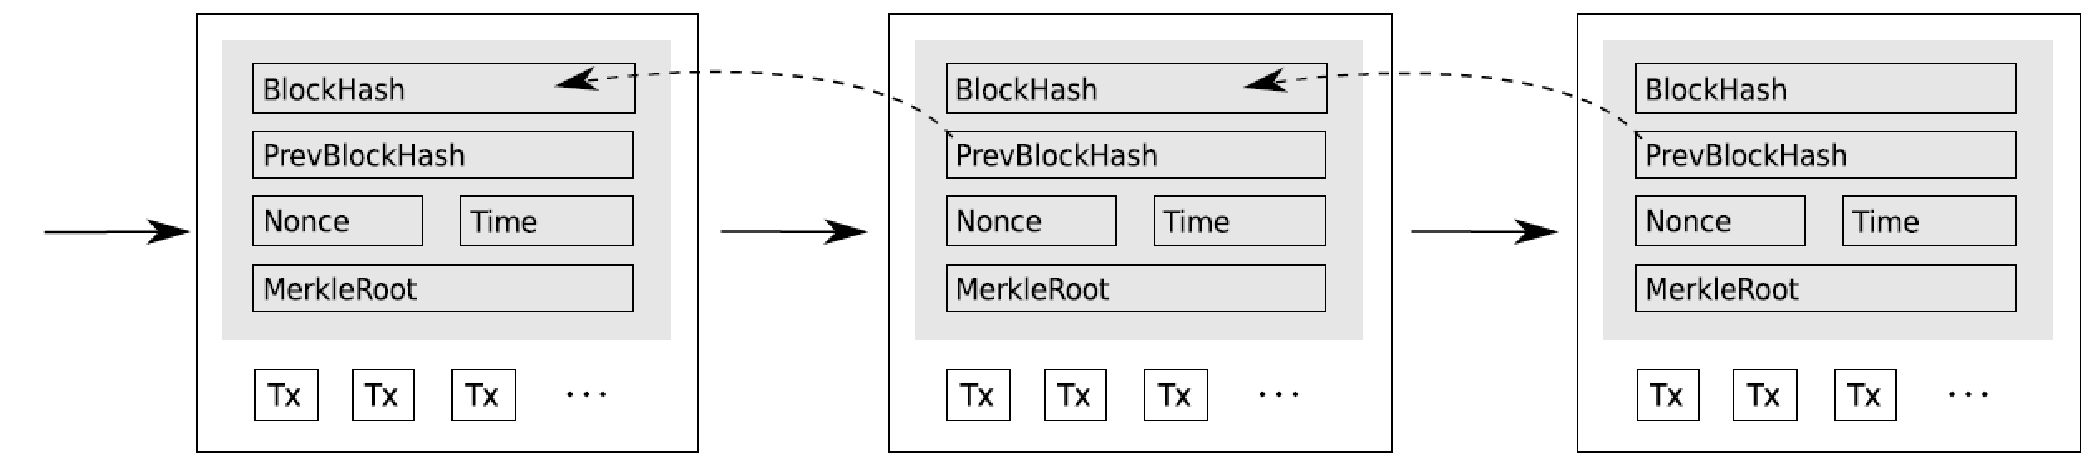
\includegraphics[width=\linewidth]{Images/Blockchain.jpg}
    \caption{Blockchain}
    \label{fig:blockchain}
\end{figure}

\section{Transaction Models: UTXO vs. Account-Based}

The strategic choice of a transaction model fundamentally shapes a blockchain's capabilities, scalability, and support for complex operations like smart contracts. The method used to track ownership and transfer value dictates how balances are calculated and how transactions are processed. The Unspent Transaction Output (UTXO) model and the Account-Based model represent the two dominant paradigms in distributed ledger technology.

\begin{table}[h!]
\centering
\begin{tabular}{|p{0.2\textwidth}|p{0.35\textwidth}|p{0.35\textwidth}|}
\hline
Feature & UTXO Model (e.g., Bitcoin) & Account-Based Model (e.g., Ethereum) \\ \hline
\textbf{Core Concept} & The ledger is a collection of unspent outputs (UTXOs) from past transactions. Ownership is tracked via these discrete pieces of value. & The ledger is a database of accounts, each with a specific state that includes a balance. \\ \hline
\textbf{Balance Calculation} & A user's balance is the sum of all UTXOs locked to their identity (address). It is not stored explicitly but calculated from available UTXOs. & A user's balance is a direct field within their account's state, which is explicitly stored and updated by transactions. \\ \hline
\textbf{Transaction Structure} & A transaction consumes one or more existing UTXOs as inputs and creates new UTXOs as outputs. & A transaction specifies a sender, a receiver, and an amount, which directly modifies the balances of the respective accounts. \\ \hline
\textbf{Smart Contract Support} & The stateless, coin-based nature of the UTXO model is ill-suited for managing the complex, multi-transactional state changes inherent to smart contracts, which are more naturally handled by the account model's explicit state transitions. & Fully supported. Transactions can be easily encoded within a smart contract to trigger complex state transitions and interactions. \\ \hline
\textbf{Transaction Processing} & Allows for parallel processing of transactions, as UTXOs are independent of one another, which can enhance scalability. & State management is generally more complex and often implemented using NoSQL databases. \\ \hline
\end{tabular}
\end{table}

In the \textbf{Unspent Transaction Output (UTXO)} model, the process of transferring value resembles handling physical cash. (See figures ~\ref{fig:UTXO_transaction_structure} and ~\ref{fig:UTXO_transactions_example})

\begin{figure}
    \centering
    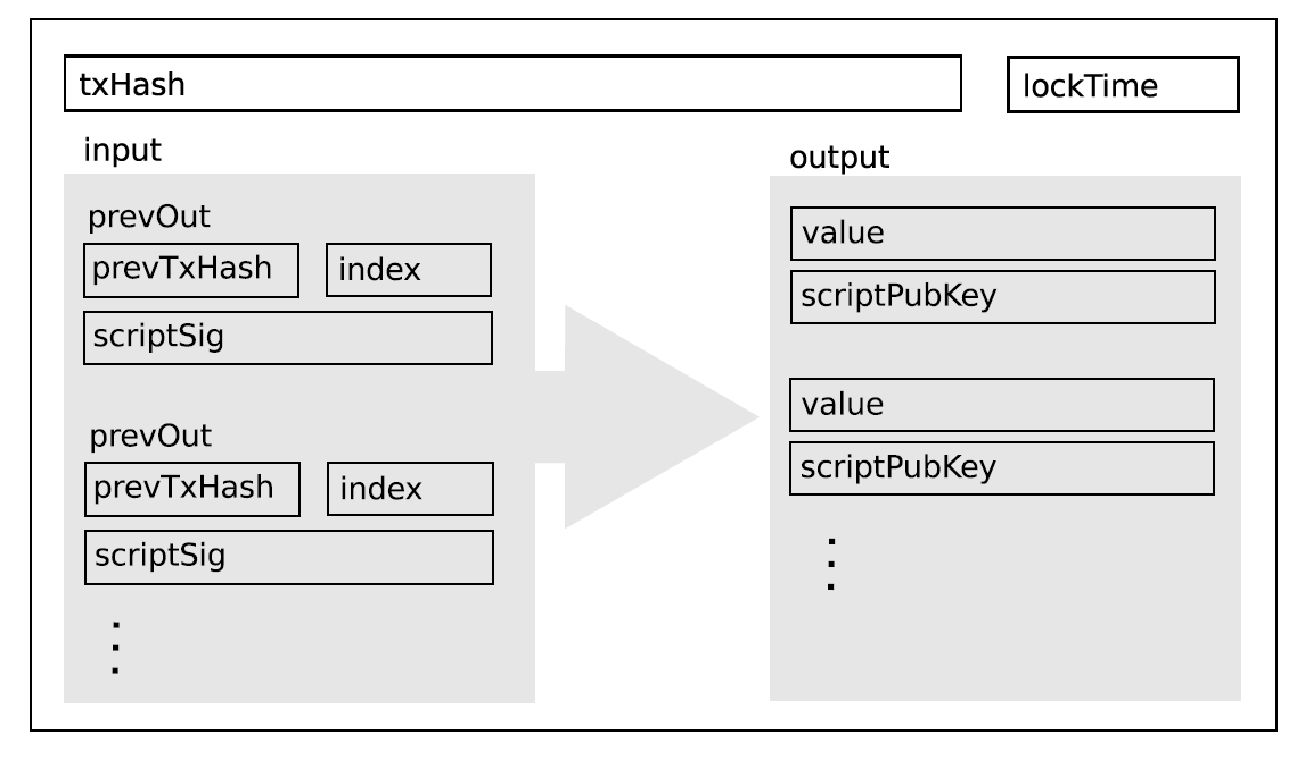
\includegraphics[width=\linewidth]{Images/UTXO_transaction_Structure.jpg}
    \caption{UTXO transaction structure}
    \label{fig:UTXO_transaction_structure}
\end{figure}

\begin{figure}
    \centering
    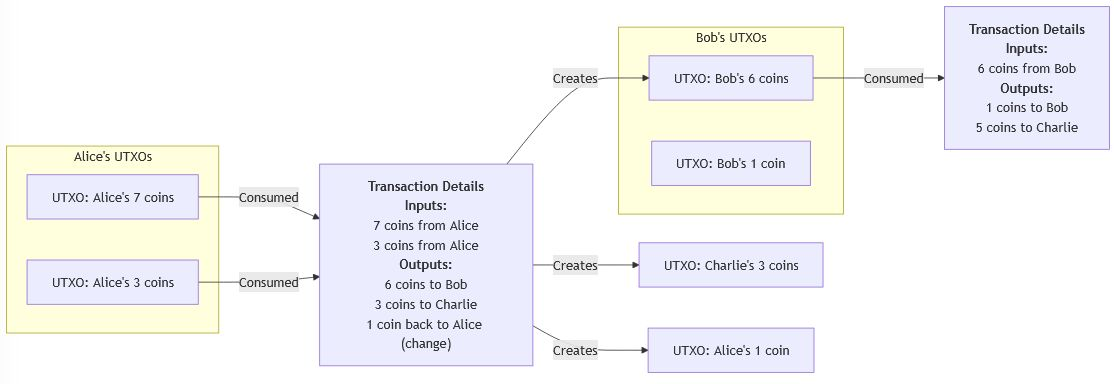
\includegraphics[width=\linewidth]{Images/UTXO_transactions_example.jpg}
    \caption{UTXO transactions example}
    \label{fig:UTXO_transactions_example}
\end{figure}

\begin{enumerate}
    \item A transaction consumes one or more existing UTXOs as \textbf{inputs}.
    \item Each input must reference a previous, unspent output by its unique transaction hash and its index within that transaction's list of outputs.
    \item The transaction then creates new \textbf{outputs}, which become new UTXOs that can be spent in future transactions.
    \item Outputs cannot be split. An entire UTXO must be consumed as an input. If the value of the UTXO is greater than the amount being sent, the remainder is sent back to the sender in a new "change" output.
    \item The total balance of a user is the sum of all UTXOs locked to their identity. This collection of all spendable outputs across the network is known as the \textbf{UTXO set}.
\end{enumerate}

The \textbf{transaction fee} in the UTXO model is not an explicit field but is implicitly calculated as:

\begin{center}
$Fee = Sum(Inputs) - Sum(Outputs)$
\end{center}

This remainder, which is not assigned to any specific output, is collected by the network participants (miners) as a reward for validating the transaction and including it in a block.\\

Security in the UTXO model is managed by "locking" and "unlocking" outputs. The most common mechanism is the \textbf{Pay-to-Public-Key-Hash (P2PKH)} script.

\begin{itemize}
    \item An output is "locked" with a script containing the cryptographic hash of the recipient's public key.
    \item To "unlock" and spend this output in a new transaction, the recipient must provide two pieces of information in the transaction's input: their original public key and a valid digital signature created with their corresponding private key.
    \item The network verifies the transaction by first checking that the provided public key hashes to the same value contained in the locking script. It then uses the public key to verify the digital signature. This process proves ownership and authorizes the spending of the UTXO without ever exposing the user's private key. This verification is not a monolithic check but a sequence of operations executed by the network using script opcodes, such as \texttt{OP\_HASH160} to hash the provided public key and \texttt{OP\_EQUALVERIFY} to compare it against the lock, followed by \texttt{OP\_CHECKSIG} to validate the digital signature.
\end{itemize}

While transaction models define how value is transferred, efficiently verifying the integrity of thousands of transactions within a single block requires another critical data structure: the Merkle tree.

\section{Ensuring Data Integrity: Merkle Trees}

A single block in a blockchain can contain thousands of transactions, presenting a significant challenge: how can the network efficiently verify the integrity of this large dataset without processing every single transaction? The Merkle tree, also known as a hash tree, provides an elegant solution to this problem by creating a single, compact cryptographic summary of all transactions in a block. (See figure ~\ref{fig:merkle_tree})\\

\begin{figure}
    \centering
    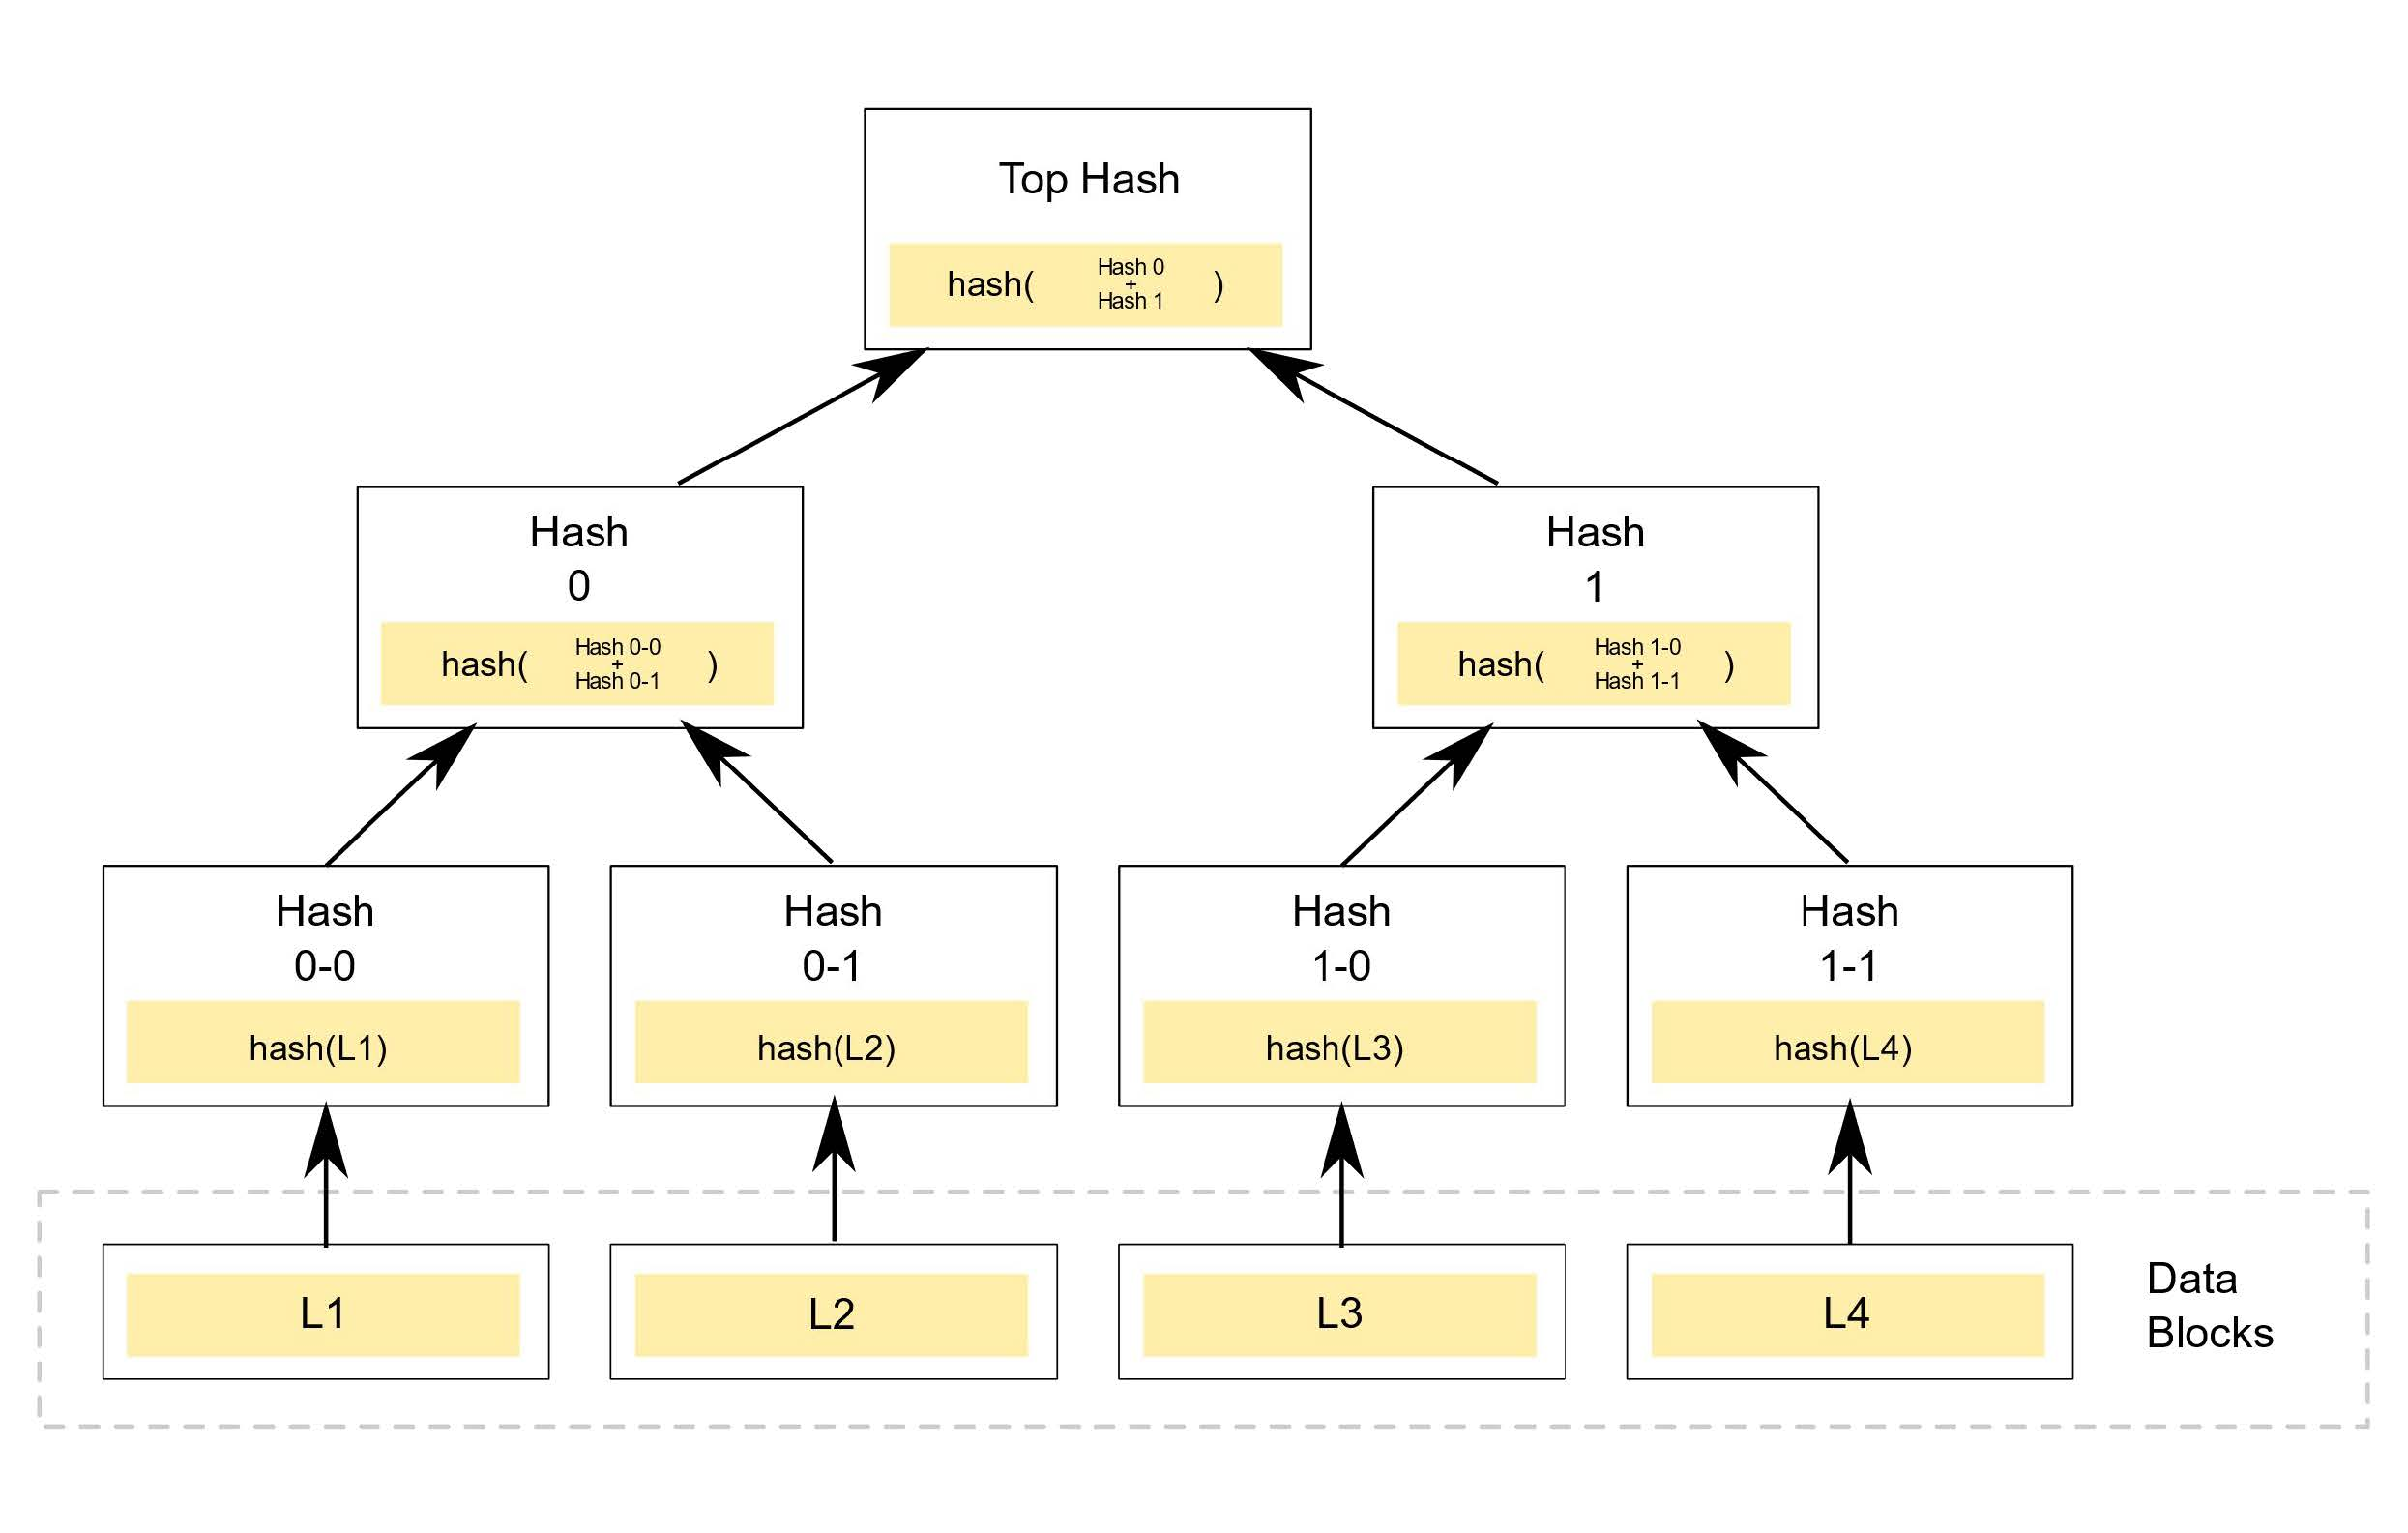
\includegraphics[width=\linewidth]{Images/Merkle_tree.jpg}
    \caption{Merkle tree}
    \label{fig:merkle_tree}
\end{figure}

\newpage

The construction of a Merkle tree is a recursive hashing process:

\begin{enumerate}
    \item Each individual transaction in the block is cryptographically hashed. These hashes form the "leaf" nodes at the bottom of the tree.
    \item Adjacent pairs of leaf nodes are concatenated and hashed together, creating a parent node on the level above.
    \item If there is an odd number of nodes at any level, the last node is duplicated and then hashed with itself to maintain a balanced tree structure.
    \item This process of pairing, concatenating, and hashing is repeated level by level, moving up the tree until only a single hash remains. This final hash is the \textbf{Merkle Root}.
\end{enumerate}

Only this single Merkle Root is stored in the block header. This design has a profound impact on data integrity: if even a single character in any transaction is altered, its corresponding leaf hash will change. This change will cascade up the tree, altering every parent hash along its path and ultimately resulting in a completely different Merkle Root. This change would invalidate the block header and, by extension, the entire block, thus securely connecting the header to every transaction within it.\\

Furthermore, Merkle trees enable highly efficient \textbf{Transaction Verification using Merkle Proofs} (See figure ~\ref{fig:merkle_proof}). To verify if a specific transaction is included in a block, a user does not need to download and process all transactions. Instead, they only need a \textbf{Merkle Proof}, which consists of the transaction’s hash and the chain of sibling hashes along the path from the transaction's leaf node to the root. To verify, a lightweight node takes the hash of the transaction in question, concatenates it with the first sibling hash provided in the proof, and hashes the result. This new hash is then concatenated with the next sibling hash at the level above, and the process is repeated up the tree. If the final computed hash matches the Merkle Root stored in the block header, the transaction's inclusion is cryptographically proven. This allows for verification with a number of computations proportional to the logarithm of the number of transactions (O(log n)), making it incredibly efficient.\\

\begin{figure}
    \centering
    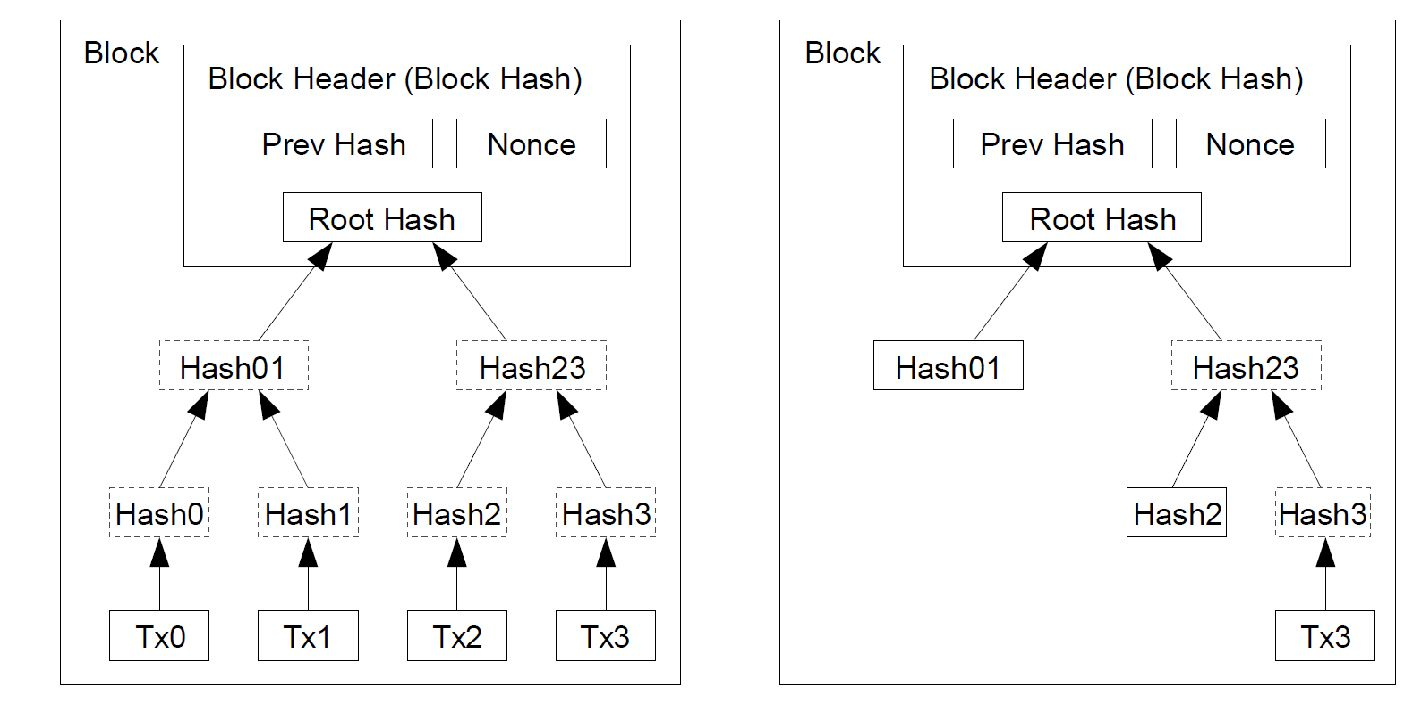
\includegraphics[width=\linewidth]{Images/Merkle_proof.jpg}
    \caption{Merkle proof}
    \label{fig:merkle_proof}
\end{figure}

This efficiency of Merkle proofs is not merely theoretical; it is the fundamental mechanism that enables the tiered network architecture, allowing Lightweight Nodes to securely verify transactions without the immense storage overhead of an Archival Full Node.

\section{Mathematical principles and implementation of the Merkle Tree}
\label{sec:merkle_tree_math}

The structure of a balanced binary Merkle Tree follows a clear mathematical relationship. The number of leaves ($y$), which corresponds to the number of transactions, and the tree's depth ($d$), which is the number of levels, are related by the following formulas:

\begin{center}
$y = 2^d$ \\
$d = log_2(y)$
\end{center}

This elegant relationship, however, introduces an implementation challenge: the number of transactions in a block is rarely a perfect power of two. To construct a balanced binary tree (See figure ~\ref{fig:Balanced_binary_tree}), the set of leaf nodes must be adjusted through a specific balancing process:

\begin{enumerate}
    \item \textbf{If the number of leaves is odd:} Duplicate the final leaf node and append it to the list. Repeat this process until the total number of leaves is a power of two.
    
    \item \textbf{If the number of leaves is even (but not a power of two):} Take the final two leaf nodes in the list and append duplicates of them (as a pair) to the list. Repeat this until the total number of leaves is a power of two.
\end{enumerate}

This two-step procedure ensures the set of leaves can always be symmetrically paired from the bottom up, allowing a complete and balanced Merkle Tree to be constructed for any number of transactions.

\begin{figure}
    \centering
    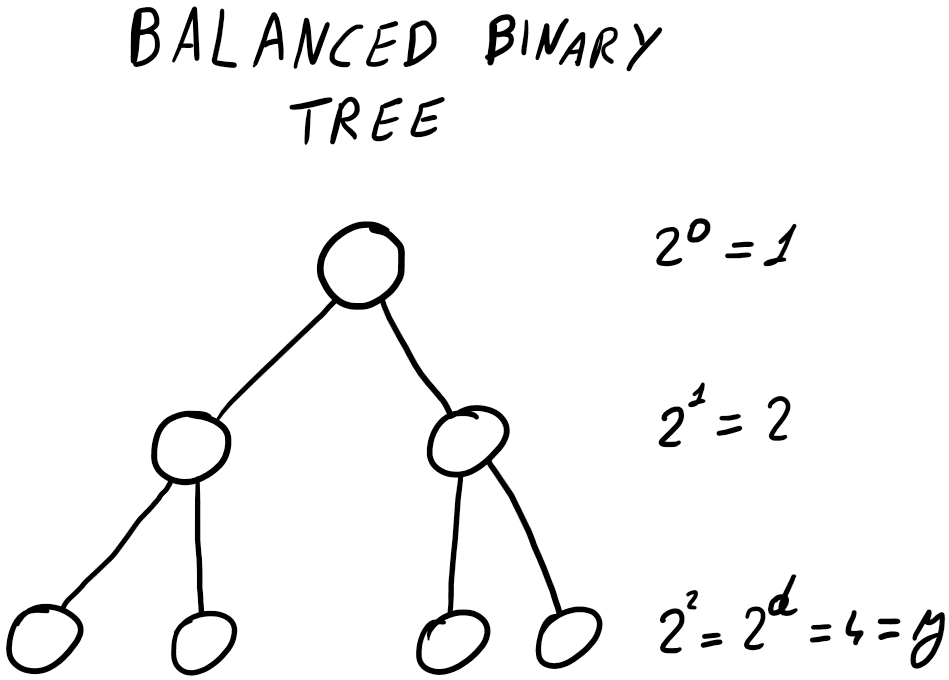
\includegraphics[width=\linewidth]{Images/Balanced_binary_tree.png}
    \caption{Balanced binary tree}
    \label{fig:Balanced_binary_tree}
\end{figure}

\section{Network Architecture and Node Types}

A blockchain is not a monolithic entity but a decentralized network of communicating computers, or nodes, each running the blockchain's software. To create an efficient and scalable network, not all nodes are required to perform the same functions. They can be categorized based on the amount of data they store and the validation tasks they perform, resulting in a tiered architecture that accommodates a wide range of participants.

\begin{itemize}
    \item \textbf{Full Node:} A full node is an active participant in the network that enforces the system's rules. It downloads and validates every block and transaction against the blockchain's consensus protocol. By doing so, full nodes maintain the security and integrity of the network without having to trust any other participant. There are two main types of full nodes:
    \begin{itemize}
        \item \textit{Archival Node:} This is a full node that downloads and stores a complete, historical copy of the entire blockchain from the very first block to the present. Archival nodes serve as a backbone for the network, providing a data source for new nodes that need to sync with the blockchain's history.
        \item \textit{Pruned Node:} This is a full node that also validates all new data but discards older blocks after validation to save disk space. While it doesn't keep the full transaction history, it maintains the complete UTXO set in a separate, in-memory database (often called the \texttt{chainstate}). Because this set represents the complete collection of all currently spendable outputs, it is sufficient to validate all new transactions and blocks without requiring the full historical block data.
    \end{itemize}
    \item \textbf{Lightweight Node (or Thin Client):} A lightweight node is designed for users who need to interact with the blockchain without the significant storage and bandwidth requirements of running a full node. It does not store the entire blockchain; instead, it downloads only the block headers. To verify if a specific transaction is included in a block, it relies on full nodes to provide a Merkle Proof. While this approach is highly efficient, it introduces an element of trust, as the lightweight node must assume that the full nodes providing the information are honest.
\end{itemize}

This network architecture, built around a linear chain of blocks, is the most established model for distributed ledgers. However, alternative architectures have emerged to address different technical challenges and use cases.\\

\section{Alternative Ledger Structures: Directed Acyclic Graphs (DAGs)}

As distributed ledger technologies (DLTs) have evolved, new data structures have been proposed to overcome the scalability, latency, and transaction fee limitations of traditional blockchains. These challenges are particularly acute in high-throughput applications like the Internet of Things (IoT). The \textbf{Directed Acyclic Graph (DAG)} has emerged as a prominent alternative ledger structure designed for these environments. (See figure ~\ref{fig:dag})\\

Unlike a blockchain, which bundles transactions into blocks that are added sequentially, a DAG-based DLT allows transactions to be added directly to the graph structure. The validation mechanism is also different. Instead of relying on miners and a global consensus protocol, a DAG requires that for a new transaction to be accepted into the ledger, it must first approve two or more previous transactions. In this model, each transaction participates in securing the network, creating a flow of approvals rather than a chain of blocks.\\

The structural differences between blockchains and DAGs result in distinct performance and operational characteristics. (See table ~\ref{tbl:BC_vs_DAG})\\

\begin{table}
    \centering
    \begin{tabularx}{\linewidth}{|X|X|X|}
        \hline
        Metric & Traditional Blockchain & DAG-Based DLT \\ \hline
        \textbf{Throughput (transactions/second)} & Lower & Higher \\ \hline
        \textbf{Power Consumption} & Higher & Lower \\ \hline
        \textbf{Transaction Latency} & Higher & Lower \\ \hline
        \textbf{Scalability} & Lower & Higher \\ \hline
        \textbf{Transaction Fees} & Higher & Lower \\ \hline
        \textbf{Consensus Robustness} & Higher & Lower \\ \hline
        \textbf{Popularity} & Higher & Lower \\ \hline
    \end{tabularx}
    \caption{Traditional blockchain and DAG-based DLT comparison}
    \label{tbl:BC_vs_DAG}
\end{table}

\begin{figure}
    \centering
    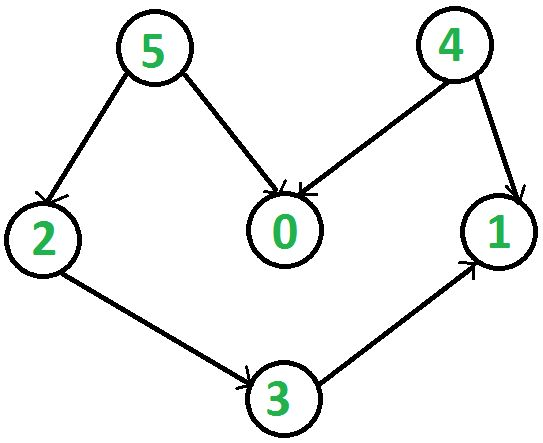
\includegraphics[width=\linewidth]{Images/DAG.jpg}
    \caption{Directed Acyclic Graph}
    \label{fig:dag}
\end{figure}

The architecture of a distributed ledger—from its transaction models and data integrity mechanisms like Merkle trees to its overarching structure as a linear chain or a directed graph—is a series of deliberate design choices. These choices collectively determine the ledger's performance, security, and ultimate suitability for specific applications, reflecting a dynamic and evolving technological landscape.

\chapter{Python implementation of a blockchain}

In this chapter we will expose a recap of the previously exposed topics and the Python codes used to develop a blockchain. These codes are just to have a better understanding of the topic and \textbf{they will not be in the exam} at least in the A.Y. 2025-2026.

\section{The Core Components: Blocks and Chains}

At its core, a blockchain is a distributed, immutable ledger. It consists of a growing list of records, called blocks, which are linked together using cryptography. Each block in the chain is a discrete data structure, and while implementations may vary, they generally contain the following core components (See figure ~\ref{fig:block_class}):

\begin{itemize}
    \item \textbf{Timestamp:} A record of when the block was created, providing a chronological anchor.
    \item \textbf{Transaction Data:} The payload of the block, which typically contains a set of validated transactions. In many systems, this data is organized into a sophisticated data structure called a Merkle Tree.
    \item \textbf{A cryptographic hash of the previous block:} This is the crucial element that connects one block to the previous.
\end{itemize}

\begin{figure}
    \centering
    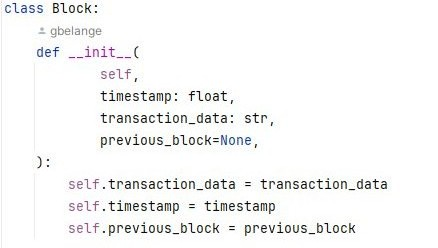
\includegraphics[width=0.5\linewidth]{Images/Block_class.jpg}
    \caption{Python block class}
    \label{fig:block_class}
\end{figure}

The inclusion of the \textit{previous block's hash} is what creates the "chain." This design, often implemented using an object-oriented approach, forges a link that is both chronological and cryptographically secure (See figure ~\ref{fig:previous_block_hash}). Each new block points back to the one that came before it by containing a unique and tamper-evident fingerprint of that preceding block. Any attempt to alter the data in a past block would change its hash, which would in turn invalidate the hashes of all subsequent blocks, making such tampering immediately obvious to the entire network. \\

This immutable linkage is made possible by cryptographic hash functions, with \texttt{\textbf{SHA-256}} being a common standard. A hash function takes an input of any size and produces a fixed-size string of characters, known as a hash. The process is deterministic (the same input always produces the same output) but irreversible. \texttt{SHA-256} generates a unique, 256-bit hash for the contents of each block, ensuring the integrity and immutability of the entire chain. (See figure ~\ref{fig:calculate_hash})\\

While the chain provides the crucial linkage \textit{between} blocks, the transaction data \textit{within} each block also requires a sophisticated structure to ensure efficiency and enable rapid verification.

\begin{figure}
    \centering
    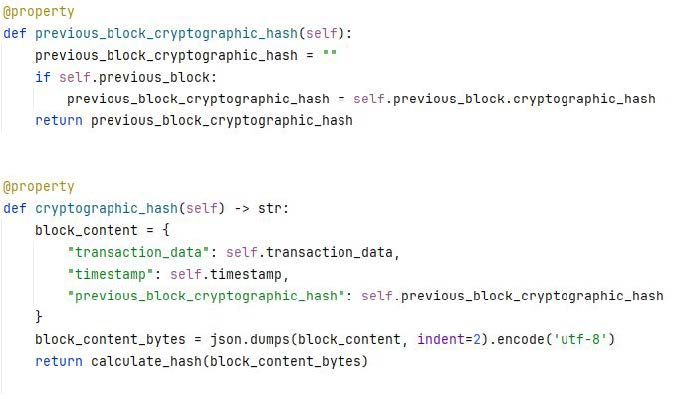
\includegraphics[width=0.5\linewidth]{Images/Previous_block_hash.jpg}
    \caption{Chain creation through the inclusion of the previous hash in the block}
    \label{fig:previous_block_hash}
\end{figure}

\begin{figure}
    \centering
    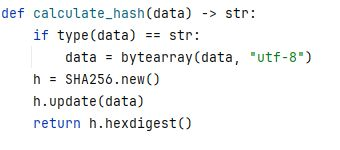
\includegraphics[width=0.5\linewidth]{Images/Calculate_hash.jpg}
    \caption{Hash computation function}
    \label{fig:calculate_hash}
\end{figure}

\section{Organizing Transactions: The Merkle Tree}

The standard method for aggregating transactions within a block is a data structure known as the \textbf{Merkle Tree}. Its use is of strategic importance, as it provides a solution for achieving efficiency, security, and scalability in a distributed network where not all participants may have the resources to store the entire history of transactions.\\

A Merkle Tree is a balanced binary tree in which every leaf node contains the cryptographic hash of a single data block (in this case, a transaction), and every non-leaf node contains the cryptographic hash of the concatenated hashes of its two child nodes. This process continues up the tree until a single hash, the "Merkle root", is generated at the top. This root hash serves as a compact and secure summary of all the transactions included in the block. To make sure that the binary tree is balanced, the generation of the tree needs to address the cases in which the number of leaves is odd or even but not a power of $2$ through a self balancing process. \\

Now, let us expose the Python implementation of the Merkle Tree referring to the file \href{https://github.com/gruyaume/my-blockchain/blob/merkle/src/node/merkle_tree.py}{merkle\_tree.py}. \\

The file contains a class with only the constructor method: the Node class.

\begin{lstlisting}[language=Python, caption={Node class}]
    class Node:
        def __init__(self, value: str, left_child=None, right_child=None):
            self.value = value
            self.left_child = left_child
            self.right_child = right_child
\end{lstlisting}

Each node contains:

\begin{itemize}
    \item A cryptographic hash value (called "value" in the code).
    \item A reference to a left child node.
    \item A reference to a right child node.
\end{itemize}

The node references have a default value of \texttt{None} to address the cases of the leaf nodes which do not have child elements and also to make the class easier to use later. \\

Before we start actually building the Merkle Tree, we need to implement a balancing process to make sure that the resulting number of leaves is a perfect power of $2$. \\

We implement the following two utility functions to use them later in the tree balancing function.

\begin{lstlisting}[language=Python, caption={Utility functions}]
    def compute_tree_depth(number_of_leaves: int) -> int:
        return math.ceil(math.log2(number_of_leaves))
    
    
    def is_power_of_2(number_of_leaves: int) -> bool:
        return math.log2(number_of_leaves).is_integer()
\end{lstlisting}

To understand the \texttt{compute\_tree\_depth} function we need to recall the mathematical relationship between the number of leaf nodes ($y$) and the depth of the tree ($d$).

\begin{center}
$y = 2^d$ \\
$d = log_2(y)$
\end{center}

The \texttt{compute\_tree\_depth} uses the second relationship and calculate its ceiling approximation in case the depth is not an integer value. For example, let's say that we have $7$ transactions in the block. We have that $log_2(7) \approx 2.8$. We expect the balancing process to add a leaf node to reach $8$ which is a perfect power of $2$. So, after the balancing process, we will have $log_2(8) = 3$ which is exactly $\lceil log_2(7) \rceil$. In conclusion, the ceiling approximation is to calculate the depth of the resulting balanced binary tree after the balancing process. \\

The function \texttt{is\_power\_of\_2} calculates the logarithm of base $2$ of the number of leaves and checks if it is a perfect integer value. \\

Now we can move on to the actual balancing function (The original function uses identifiers referring to nodes, but they are meant to be hashes. In fact, the Merkle Tree building function will use the data as the values of the nodes which means that they are hashes, not nodes.):

\begin{lstlisting}[language=Python, caption={Tree balancing function}]
    def fill_set(list_of_hashes: list):
        current_number_of_hashes = len(list_of_hashes)
    
        # In this case we don't need to do anything
        if is_power_of_2(current_number_of_hashes):
            return list_of_hashes
    
        # We calculate the target number of leaves y as 2^d
        total_number_of_hashes =
            2 ** compute_tree_depth(current_number_of_hashes)
    
        # We add leaf nodes to the tree distinguishing
        # the two imbalanced tree cases.
    
        # The number of leaves is even but not a power of 2
        if current_number_of_hashes % 2 == 0:
            for i in range(current_number_of_hashes,
                            total_number_of_hashes, 2):
                list_of_hashes =
                    list_of_hashes + [list_of_hashes[-2],
                        list_of_hashes[-1]]
    
        # The number of leaves is odd
        else:
            for i in range(current_number_of_hashes,
                    total_number_of_hashes):
                list_of_hashes.append(list_of_hashes[-1])
    
        return list_of_hashes
\end{lstlisting}

The balancing function takes in input the list of hashes and calculates its length as a first operation. Before we proceed, we need to make sure that the number of hashes is not already a perfect power of $2$ because, in such case, we don't have to do anything and we can return the list of hashes as is. \\

If the number of hashes is not a perfect power of $2$, we calculate the target number of hashes using the relation $y = 2^d$ and the \texttt{compute\_tree\_depth} function. Now that we have the target number of hashes we need to add hashes to the list to reach the target length. We recall that the balancing process consists of the following operations:

\begin{enumerate}
    \item \textbf{If the number of leaves is odd:} Duplicate the final leaf node and append it to the list. Repeat this process until the total number of leaves is a power of two.
    
    \item \textbf{If the number of leaves is even (but not a power of two):} Take the final two leaf nodes in the list and append duplicates of them (as a pair) to the list. Repeat this until the total number of leaves is a power of two.
\end{enumerate}

\newpage

Now, let us expose the actual Merkle Tree building function.

\begin{lstlisting}[language=Python, caption={Function to build the Merkle Tree}]
    def build_merkle_tree(node_data: [str]) -> Node:
        complete_set = fill_set(node_data)
        old_set_of_nodes = [Node(calculate_hash(data)) for data in complete_set]
        tree_depth = compute_tree_depth(len(old_set_of_nodes))
    
        for i in range(0, tree_depth):
            num_nodes = 2**(tree_depth-i)
            new_set_of_nodes = []
            for j in range(0, num_nodes, 2):
                child_node_0 = old_set_of_nodes[j]
                child_node_1 = old_set_of_nodes[j+1]
                new_node = Node(
                    value=calculate_hash(f"{child_node_0.value}{child_node_1.value}"),
                    left_child=child_node_0,
                    right_child=child_node_1
                )
                new_set_of_nodes.append(new_node)
            old_set_of_nodes = new_set_of_nodes
        return new_set_of_nodes[0]
\end{lstlisting}

This function takes the list of hashes in input and returns the Merkle Root as the output. As a first operation, we make sure that the length of the list of hashes is a power of two using the \texttt{fill\_set} function. Once we have an appropriate list of hashes, we can use it to create a list of nodes and we can use the length of the list of nodes to calculate the depth of the Merkle Tree. \\

At this point we can use a for loop to generate the tree from the bottom to the top. First, we calculate the number of nodes at the current level of the tree and we initialize the list of nodes at the higher level as an empty list. Then, we use a nested for loop to retrieve the nodes at the current level two at a time and generate their parent node. We set the references to the child nodes and we use the concatenation of their hash values to calculate the hash value of the parent. Once we have the parent node, we append it to the list of nodes at the higher level. \\

After the inner for loop, the value of the new set of nodes becomes the value of the old set of nodes for the following iteration. And after the outer for loop we can retrieve the Merkle Root as the first (only) node contained in the list of nodes at the higher level. \\

To have a better understanding of the function, let us apply it to the balanced binary tree we exposed in section ~\ref{sec:merkle_tree_math}. (See figure ~\ref{fig:Balanced_binary_tree}) \\

The list of hashes contains $4$ elements and $4$ is a power of $2$. This means that, in this case, the variable \texttt{complete\_set} is equal to the variable \texttt{node\_data} because the function \texttt{fill\_set} does not add elements. We generate the list of nodes and we compute $d = log_2(y) = 2$. \\

As for the outer loop, we have that \texttt{range(0, tree\_depth) = [0, 1]} so, we have $2$ iterations:

\begin{enumerate}
    \item In this iteration we have that $i=0$ and $num\_nodes = 2^{(d-0)} = 2^2 = 4$. This means that the inner for loop iterates two times to calculate the nodes at the higher level.

    \item In this iteration we have that $i=1$ and $num\_nodes = 2^{(d-1)} = 2^1 = 2$. This means that the inner for loop iterates only once to calculate the Merkle Root which is in the position $0$ of the list \texttt{new\_set\_of\_nodes}.
\end{enumerate}

\section{Identities and Wallets}

Now let us expose the Python implementation of the wallet that we can find in the file \href{https://github.com/gruyaume/my-blockchain/blob/utxo/src/wallet/wallet.py}{wallet.py}. This file, in addition to the codes we are about to expose, also contains the \texttt{Transaction} class that we will expose in subsection ~\ref{sec:transaction}. \\

The file starts with the definition of the \texttt{Owner} class which only has the constructor method (See figure ~\ref{fig:owner_class}). A user's identity on the network is defined by a set of cryptographic keys, which are typically managed by a software application known as a wallet. The core components are:

\begin{enumerate}
    \item A \texttt{\textbf{private key}}, a secret number that grants the owner the authority to spend their funds.
    \item A \texttt{\textbf{public key}}, which is mathematically derived from the private key.
    \item An \texttt{\textbf{address}} (called \texttt{public\_key\_hash} in the code), which serves as the public identifier where funds can be sent.
\end{enumerate}

\begin{figure}
    \centering
    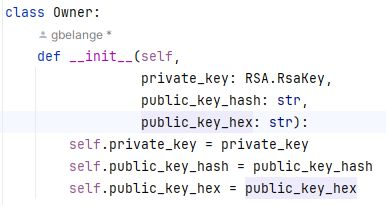
\includegraphics[width=0.5\linewidth]{Images/Owner_class.jpg}
    \caption{Owner class}
    \label{fig:owner_class}
\end{figure}

After the \texttt{Owner} class we can find the \texttt{initialize\_wallet} function (See figure ~\ref{fig:initialize_wallet}).
In this function we generate the values contained in the \texttt{Owner} class. We start by generating a private key using the RSA algorithm and deriving its relative public key. Then, we calculate an hexadecimal representation of the public key because the \texttt{Owner} class requires it and we convert it into a Python string using the \texttt{decode("utf-8")} method.
The address is generated from the hexadecimal public key through a double-hashing process designed to provide both security and a shorter, more manageable identifier. First, the public key is hashed using the \texttt{SHA-256} algorithm which produces a digest of 64 hexadecimal characters. The result of that hash is then hashed again, this time using the \texttt{RIPEMD160} algorithm whose deigest is 40 hexadecimal characters long. This final \texttt{RIPEMD160} hash is the user's public address.

\begin{figure}
    \centering
    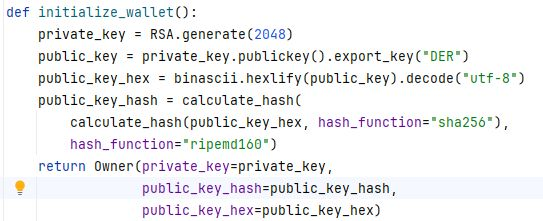
\includegraphics[width=0.5\linewidth]{Images/Initialize_walet.jpg}
    \caption{Initialize wallet function}
    \label{fig:initialize_wallet}
\end{figure}

\section{Representing Ownership: The UTXO Model and Transaction Anatomy}

Unlike traditional banking systems which rely on an "account-based" ledger that tracks balances, foundational cryptocurrencies like Bitcoin introduced a different accounting method: the \textbf{Unspent Transaction Output (UTXO)} model. In this model, there is no concept of an account balance. Instead, the blockchain tracks individual pieces of currency—the unspent outputs of past transactions—which are scattered across the ledger and controlled by their respective owners.

\subsection{The Anatomy of a Transaction}
\label{sec:transaction}

\begin{figure}
    \centering
    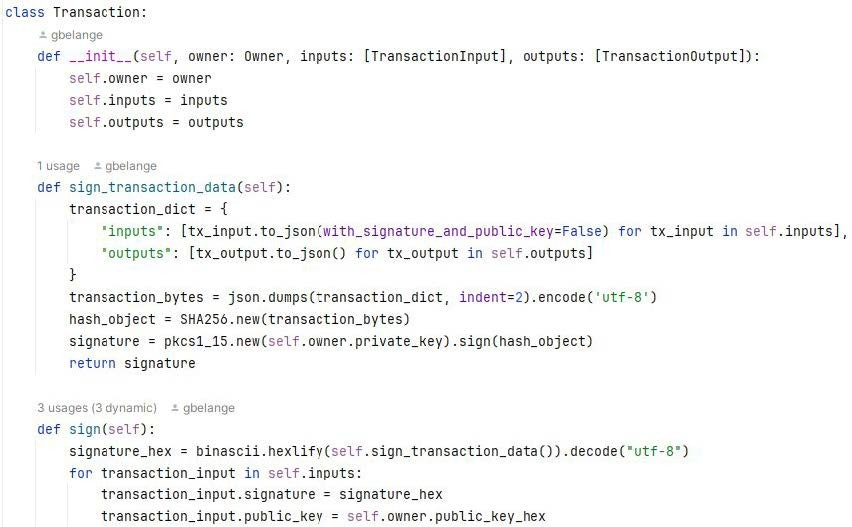
\includegraphics[width=0.5\linewidth]{Images/Transaction.jpg}
    \caption{Transaction class}
    \label{fig:transaction_class}
\end{figure}

A transaction is a data structure that facilitates the transfer of value on the blockchain (See figure ~\ref{fig:transaction_class}). It is fundamentally composed of inputs and outputs. We define them in classes because each transaction object can have more than one input and output object. (See figures ~\ref{fig:transaction_input} and ~\ref{fig:transaction_output})

\begin{itemize}
    \item \textbf{Transaction Owner:} The \texttt{Owner} object representing the identity of the user who issued the transaction.

    \item \textbf{Transaction Inputs:} These are pointers to UTXOs from previous transactions that the sender now wishes to spend. Each input must specify:
    \begin{itemize}
        \item The transaction ID of a past transaction containing the UTXO (\texttt{transaction\_hash} in the code).
        
        \item The index of the specific output from that past transaction which is now being spent. (The union of the transaction ID and the output index uniquely identifies the output of the past transaction being used as input for the current one)

        \item The public key of the owner of the output (To identify the user).
        
        \item A digital signature generated with the owner's private key (To certify that the transaction was issued by the user).
    \end{itemize}
    
    \item \textbf{Transaction Outputs:} These are the new UTXOs being created by the transaction. Each output contains:
    \begin{itemize}
        \item The value or amount of currency being transferred.
        \item The public key hash (address) of the recipient, who will be the sole party able to spend this new UTXO in the future.
    \end{itemize}
    
    \item \textbf{Digital sign method:} The Transaction class provides methods to digitally sign the transaction. This is the critical component that authorizes the spending of funds. To generate it, a string representation of the transaction's data (grouping its inputs and outputs, called \texttt{transaction\_bytes} in the code) is created and then hashed with \texttt{SHA-256}. This hash is then "signed" using the owner's private key. This unique signature is included in each transaction input, providing cryptographic proof that the owner of the funds has authorized the transaction. Any node can verify the signature using the public key included in the input, ensuring authenticity and integrity of the transaction.
\end{itemize}

\begin{figure}
    \centering
    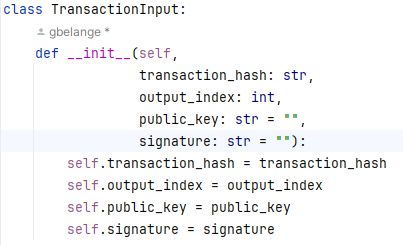
\includegraphics[width=0.5\linewidth]{Images/Transaction_input.jpg}
    \caption{Transaction input class}
    \label{fig:transaction_input}
\end{figure}

\begin{figure}
    \centering
    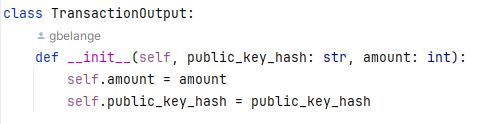
\includegraphics[width=0.5\linewidth]{Images/Transaction_output.jpg}
    \caption{Transaction output class}
    \label{fig:transaction_output}
\end{figure}

These fundamental data structures—blocks, chains, Merkle Trees, and transactions—represent the \textit{what} of a blockchain: the data itself and how it is organized. In the next part, we will explore the \textit{how}: the dynamic and complex process by which a global network of independent nodes agrees on the state of this shared data.

\end{document}
